\documentclass[10pt,letterpaper]{article}

% Template selection.
% Uncomment exactly one pair: \XXtrue + \XXfalse for the others.

\newif\ifarxiv
\newif\ifmlsys

% arXiv (default) — PRIMEarxiv style
\arxivtrue
\mlsysfalse

% MLSys — uncomment and comment out the arXiv block above
% \arxivfalse
% \mlsystrue


\ifarxiv
  \usepackage{PRIMEarxiv}
\fi
\ifmlsys
  % \usepackage{mlsys} % uncomment and provide mlsys.cls when targeting MLSys
\fi

\usepackage[utf8]{inputenc}
\usepackage[T1]{fontenc}
\usepackage{hyperref}
\usepackage{url}
\usepackage{booktabs}
\usepackage{array}
\usepackage{amsfonts}
\usepackage[expansion=false]{microtype}
\usepackage{graphicx}
\usepackage{amsmath,amssymb}
\usepackage[table]{xcolor}
\usepackage{tikz}
\usepackage{pgfplots}
\usetikzlibrary{shapes.geometric,arrows,positioning,calc}
\pgfplotsset{compat=1.18}

\usepackage{listings}
\lstset{%
  basicstyle=\ttfamily\small,
  breaklines=true,
  frame=single,
}

\def\figdir{figures}
\definecolor{tensoraSync}{HTML}{D8ECFF}
\definecolor{tensoraAsync}{HTML}{E5F5E0}
\definecolor{tensoraUring}{HTML}{FEE8C8}
\newcommand{\syncwin}{\cellcolor{tensoraSync}\texttt{sync}}
\newcommand{\asyncwin}{\cellcolor{tensoraAsync}\texttt{async}}
\newcommand{\uringwin}{\cellcolor{tensoraUring}\texttt{io\_uring}}

\hypersetup{%
  pdftitle={Evaluating I/O Backends for LLM Checkpoint Loading Across Formats, Layers, and Environments},
  pdfauthor={Botir Khaltaev},
  pdfkeywords={large language models, checkpoint loading, I/O backends, io\_uring, cold start, vLLM, evaluation, systems measurement}%
}

%% Title
\title{Evaluating I/O Backends for LLM Checkpoint Loading Across Formats, Layers, and Environments}

%% Authors
\author{
  Botir Khaltaev\\
  Independent, United Kingdom\\
  \texttt{btrghstk@gmail.com}
}

\begin{document}
\maketitle

\begin{abstract}
Cold-start latency in large language model (LLM) serving is usually treated as a bandwidth problem: how quickly can storage stream checkpoint bytes to GPU memory? This paper argues that the dominant factor is not peak throughput but the interaction between \emph{checkpoint layout, I/O backend, and integration layer}. A checkpoint layout determines the file and range requests exposed to the operating system; an I/O backend determines how those requests are submitted and completed; Python bindings and serving engines determine how much of any backend gain reaches the user. Consequently, no single I/O backend dominates across the full parameter space.

We present a systematic evaluation using Tensora, an open checkpoint-loading framework designed for backend attribution. We compare sync, async (Tokio), and Linux \texttt{io\_uring} across two layouts (contiguous SafeTensors shards and a partitioned ServerlessLLM-style layout), six public checkpoints from 0.6B to 32B parameters, two measured layers (Rust backend attribution and vLLM integration), and four environments (H100 with local NVMe, H200 and A100 with blocked \texttt{io\_uring}, Modal H100 under gVisor). Held-out validation on Mistral-7B-Instruct confirms that regime structure generalises beyond the primary model ladder. Representative single-run screening on H100, H200, and A100 provides broad regime coverage; repeated five-repetition anchoring on the Modal H100 environment provides complementary variance evidence in a restricted container setting.

Four findings emerge. First, H100 SafeTensors loading exhibits a scale crossover: sync is fastest for small models (0.6B to 4B); \texttt{io\_uring} is fastest from 8B through 32B (1.28$\times$ over sync at 32B). Second, on H100, sync is never the fastest backend on the ServerlessLLM layout; async and \texttt{io\_uring} trade places by partition structure and scale. Third, integration layers reorder absolute times but preserve relative backend effects: in vLLM cold \texttt{load\_only}, Tensora's \texttt{io\_uring} SafeTensors path reduces initialization by 37 to 48\% for 8B and 32B checkpoints relative to vLLM's native loader. Fourth, ordering regimes are more portable than backend identities: small-scale sync dominance transfers across environments, but the large-scale winner depends on I/O topology and kernel capability.
\end{abstract}

\keywords{large language models \and checkpoint loading \and I/O backends \and io\_uring \and cold start \and vLLM \and systems evaluation}

\section{Introduction}
\label{sec:introduction}

An LLM serving request cannot generate a token until model weights are resident. In serverless and multi-tenant settings, idle models are commonly evicted to recover scarce accelerator memory; the next request then pays a cold load before inference begins. A 7B float16 checkpoint is already on the order of 14~GB, and the checkpoints in this paper reach beyond 65~GB of weight bytes. Cold loading is therefore not a startup footnote; it is part of the user-visible serving path.

The usual shorthand is to call this a bandwidth problem. That shorthand is incomplete. A loader does not read an abstract number of gigabytes; it executes a concrete read plan. The checkpoint format decides whether bytes appear as a few contiguous shards or as many indexed ranges across partition files. The I/O backend decides whether those reads are submitted through blocking POSIX calls, an async runtime, or \texttt{io\_uring}. The integration layer then adds its own costs: Python object construction, tensor materialization, CUDA context setup, allocator initialization, and serving-engine configuration. A device can have high peak throughput and still produce poor cold-start time when request geometry and submission method are mismatched.

Existing LLM serving systems and checkpoint libraries typically treat loading as a fixed initialization cost with a single code path. No prior work, to our knowledge, systematically evaluates I/O backend choice for LLM checkpoint loading as a function of format, scale, and deployment environment. This gap matters because the optimal backend is not stable across the parameter space.

This paper evaluates three explicit I/O backends: synchronous POSIX I/O, Tokio-based async loading, and Linux \texttt{io\_uring}, across two checkpoint layouts, six model scales, four environments, and two measured layers (Rust and vLLM) with Python as the integration bridge. Our central finding is:

\begin{quote}
\textbf{No single I/O backend dominates.} The best backend depends on checkpoint layout, model scale, backend availability, and the layer at which loading is observed. A fixed rule such as ``always sync,'' ``always async,'' or ``always \texttt{io\_uring}'' leaves performance on the table.
\end{quote}

SafeTensors presents mostly whole-file or multi-shard eager loading: after metadata parsing, the loader must move large contiguous byte regions. ServerlessLLM-style partitioning presents a different workload: tensors are reconstructed from indexed partition files, creating many grouped range reads. These layouts are not cosmetic alternatives; they expose different I/O regimes. Scale then moves the boundary within a regime: a backend with low orchestration overhead can win for a small single-shard load, while a backend that sustains deeper submission queues can win for a large multi-shard load.

We built Tensora\footnote{Tensora is this paper's checkpoint-loading framework (Rust crate \texttt{tensora}, Python package \texttt{tensora\_py}). It is unrelated to Google's TensorStore library for array storage.}, an open framework for evaluating these regimes. Tensora exposes sync, async, and \texttt{io\_uring} under shared format abstractions, enabling controlled backend attribution across layers. We evaluate six public checkpoints from 0.6B to 32B parameters across two layouts and two measured layers: Rust backend attribution and a custom vLLM integration. The primary environment is an H100 host with local NVMe and working \texttt{io\_uring}; H200 and A100 container environments with network-attached storage and blocked \texttt{io\_uring} test whether ordering regimes transfer when the strongest H100 backend is unavailable. A Modal H100 environment under gVisor provides restricted-container validation.

On H100 SafeTensors, sync wins at the small end and \texttt{io\_uring} from Qwen3-8B through Qwen3-32B (1.28$\times$ over sync). On H100 ServerlessLLM, sync is never fastest; async and \texttt{io\_uring} lead different rows. vLLM reorders backend rankings (it measures a different construct) but the effect survives integration: in vLLM cold \texttt{load\_only}, Tensora's \texttt{io\_uring} SafeTensors path reduces initialization by 37 to 48\% relative to vLLM's native loader for 8B and 32B checkpoints. Cross-environment results preserve small-scale sync dominance on three of four environments while showing that the large-scale winner depends on kernel and storage context.

\textbf{Contributions.}
\begin{enumerate}
  \item \textbf{Format-driven backend dependence.} We evaluate three I/O backends (sync, async, \texttt{io\_uring}) across two checkpoint layouts and six model scales, showing that the best backend shifts systematically with format and scale: sync wins on small SafeTensors, \texttt{io\_uring} wins on large SafeTensors, and sync never wins on H100 ServerlessLLM. To our knowledge, this is the first controlled evidence that LLM checkpoint loading is workload-dependent rather than bandwidth-bound.
  \item \textbf{Backend regime persistence through integration.} We provide controlled evidence across two measured layers (Rust and vLLM) demonstrating that backend ordering regimes propagate through library and serving-engine boundaries. The proportional advantage shrinks but the regime structure survives.
  \item \textbf{Regime transfer across environments.} We validate across four environments (H100, H200, A100, Modal) that small-scale sync dominance transfers widely while the large-scale winner depends on storage topology and kernel capability. Regime structure, not backend identity, is the portable quantity.
\end{enumerate}

\section{Related Work}
\label{sec:related_work}

This section positions our thesis---that LLM checkpoint loading depends on workload shape and should be selected adaptively---against four bodies of work: serving systems, serverless cold-start systems, checkpoint formats and loading infrastructure, and operating-system I/O policy. The common gap is that prior work either optimises after weights are resident, avoids loads through caching or placement, or improves the kernel/storage substrate. Tensora measures the application-level load mechanics themselves.

\subsection{LLM Serving Systems}

Production LLM serving engines primarily optimise throughput and latency once weights are resident. vLLM introduces PagedAttention for efficient KV-cache management \cite{pagedattention}. Orca pioneers iteration-level batching \cite{orca}. Sarathi-Serve refines the prefill--decode scheduling trade-off \cite{sarathi_serve}. DeepSpeed Inference applies model parallelism and kernel fusion \cite{deepspeed_inference_paper}. These systems make the serving pipeline efficient after model initialisation; checkpoint loading is usually treated as a fixed prelude to the serving path.

Our vLLM experiments use a serving engine precisely to test whether backend effects survive that larger context. They do not replace serving-system research; they isolate a cost that serving systems usually inherit from the loader.

\subsection{Serverless Cold Start}

Serverless LLM serving makes cold start a first-order concern: idle models are evicted and must be reloaded on demand. ServerlessLLM \cite{FU:2024} proposes multi-tier loading with GPU/NVMe/DRAM placement and live migration. HydraServe \cite{hydraserve} minimises cold-start latency in public clouds through pipeline parallelism and placement optimisation. Snapshot-based warm-up approaches \cite{silva2021snapshot} pre-materialise process or model state to bypass part of startup.

These systems optimise \emph{whether}, \emph{where}, or \emph{when} loading occurs. Tensora asks a complementary question: when a load is unavoidable, which userspace submission policy moves the required bytes fastest for this checkpoint geometry? That question remains relevant even in tiered-storage systems because each tier still exposes an I/O workload to the loader.

\subsection{Checkpoint Formats and Loading Systems}

Checkpoint formats determine what byte ranges a loader must read and whether those reads are contiguous, sharded, partitioned, or fragmented. SafeTensors \cite{safetensors_docs} provides safe tensor serialisation with contiguous whole-file or multi-shard layouts. GGUF optimises for memory-mapped CPU inference and quantised deployments. ServerlessLLM's partitioned layout \cite{serverlessllm_repo} distributes tensors across partition files with a central index, enabling partial loading and tiered placement.

Recent systems work optimises the loading path from different layers. BlitzScale \cite{blitzscale} uses GPU-side model caching over NVLink and RDMA to share already-loaded models between inference instances. Most relevant to our work, PPC/MAIO \cite{fast26_maio} optimises model loading through a programmable kernel page cache, adapting prefetching and eviction to LLM I/O patterns. MAIO operates below the system-call interface; Tensora operates above it, comparing userspace I/O backends on identical logical read plans. These approaches are complementary: kernel cache policy determines how pages are served, while userspace backend policy determines how application reads are issued.

A separate line of characterization work studies LLM checkpoint/restore I/O patterns on parallel file systems \cite{arxiv2512_checkpoint_io}, covering buffered versus direct I/O paths and liburing performance. That work focuses on training checkpointing in HPC environments; our focus is inference checkpoint loading in single-node serving.

The gap we address is therefore format-conditioned backend selection: given a fixed checkpoint layout, which userspace backend and planning strategy should execute the read plan, and how does the answer change with model scale and integration layer?

\subsection{I/O Backend Policy}

The Linux I/O interface landscape spans blocking POSIX calls, asynchronous runtimes built above them, POSIX AIO, and \texttt{io\_uring}. Recent database research provides the closest methodological template for our work: Jasny et al. \cite{IOURING_DATABASE_GUIDELINES} show that \texttt{io\_uring} benefits depend on workload shape and queue depth. Bulk sequential reads may already amortise syscall overhead, while many-small or high-concurrency workloads benefit from batched submission.

LLM checkpoint loading spans both regimes. Contiguous SafeTensors shards resemble bulk sequential access with shard-level fanout. Partitioned ServerlessLLM layouts resemble grouped range workloads. Our work translates the workload-shape lesson to LLM loading and extends it with cross-layer evidence (Rust, Python, vLLM), capability-gated fallback when \texttt{io\_uring} is blocked, and an adaptive policy grounded in workload features rather than API names.

\subsection{Positioning}

We do not introduce a new checkpoint format, optimise steady-state serving throughput, or solve cluster scheduling. We measure load mechanics across four backend policies and two layouts, for six public checkpoints, at three integration layers. The contribution is operational: evidence that backend choice depends jointly on layout, scale, and availability, plus a format-aware adaptive policy with explicit overrides. This is the missing piece between format design (what bytes exist), serving engines (how loaded weights are used), and kernel-level storage optimisation (how pages are served).

\section{Tensora Design}
\label{sec:design}

Tensora is the measurement framework for this paper. Its design goal is to make workload shape, backend choice, and integration overhead explicit enough to measure across I/O backends.

\subsection{Design principles}

A format parser should produce the same read plan regardless of backend, so timing differences reflect submission mechanism rather than work performed. Backend labels are explicit at the harness level. Measurement (cache drops, timing, capture) stays outside the loader.

\subsection{Architecture}

Tensora separates format parsing, backend execution, and evaluation (Figure~\ref{fig:tensora-arch}). The \textbf{format layer} parses checkpoint metadata and produces a request-local read plan: files, byte ranges, tensor names, and expected sizes. The \textbf{backend layer} executes reads through an explicit backend (sync, async, or the adaptive default) selected by the caller. The \textbf{evaluation layer} contains the Rust profiler and vLLM experiments; Python bindings bridge the integration path.

\begin{figure}[t]
  \centering
  \resizebox{\linewidth}{!}{%
  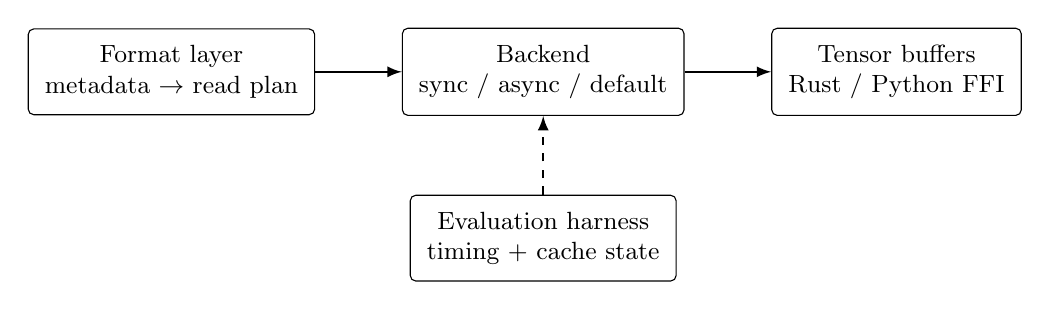
\begin{tikzpicture}[
    font=\small,
    box/.style={draw, rounded corners=2pt, align=center, inner sep=6pt, minimum width=2.6cm},
    arr/.style={->, >=latex, thick},
  ]
    \node[box] (fmt) {Format layer\\metadata $\rightarrow$ read plan};
    \node[box, right=1.1cm of fmt] (be) {Backend\\sync / async / default};
    \node[box, right=1.1cm of be] (out) {Tensor buffers\\Rust / Python FFI};
    \node[box, below=1.0cm of be] (ev) {Evaluation harness\\timing + cache state};
    \draw[arr] (fmt) -- (be);
    \draw[arr] (be) -- (out);
    \draw[arr, dashed] (ev) -- (be);
  \end{tikzpicture}%
  }
  \caption{Tensora architecture. The hot path is format parsing $\rightarrow$ backend execution $\rightarrow$ tensor buffers. The harness controls timing and cache state outside that path.}
  \label{fig:tensora-arch}
\end{figure}

All backends receive the same read plan from the format layer and execute reads through the selected I/O submission method.

\subsection{Common backend surface}

All eager backends implement the same conceptual operations:

\begin{itemize}
\item \texttt{load(path)} for one full file,
\item \texttt{load\_batch(paths)} for multiple whole-file loads,
\item \texttt{load\_range(path, offset, len)} for one byte range, and
\item \texttt{load\_range\_batch(requests)} for grouped range reads.
\end{itemize}

This surface is deliberately small. SafeTensors mostly exercises whole-file and batch loading; ServerlessLLM exercises range batches. Backend implementations may chunk, group, coalesce, or tune queue depth internally, but they must satisfy the same logical tensor plan.

\subsection{Backend implementations}

The \textbf{sync} backend uses blocking POSIX reads with practical host-side parallelism for large files. It is not a strawman serial baseline; its performance on small SafeTensors loads reflects real low-overhead bulk I/O where orchestration cost is minimal.

The \textbf{async} backend is built on Tokio. It groups work per file, batches dynamically, and avoids unnecessary task fanout. Its concurrent scheduling model amortizes per-request overhead when many operations are in flight, which becomes advantageous for larger SafeTensors workloads and for ServerlessLLM's range-dominated access pattern.

The \textbf{default} backend is an adaptive selector that chooses between sync and async (or \texttt{io\_uring} when available) based on checkpoint layout, model scale, and platform capability. It is designed to match or approach the best explicit backend at each point in the format$\times$scale space without requiring manual backend selection.

On platforms where \texttt{io\_uring} is available (bare-metal Linux with kernel $\geq$ 5.6), Tensora also exposes an \textbf{\texttt{io\_uring}} backend with persistent rings, batched submissions, and workload-dependent chunk planning. This backend is unavailable on Modal's gVisor containers (\texttt{ENOSYS}) and is therefore not part of the primary evaluation.

The mmap-backed path remains useful for lazy selective access, especially through Python handles, but it is not the main eager cold-start mechanism evaluated in the Rust matrices.

\subsection{Formats and integrations}

Tensora supports two layouts because they expose different regimes. \texttt{SafeTensors} presents whole-file or multi-shard contiguous loading. \texttt{ServerlessLLM} presents an indexed partition layout with range-oriented reads. Supporting both under one framework is what makes the layout-dependent regime claim measurable.

Python bindings are implemented with PyO3 and expose a small API: sync and async eager load, and lazy \texttt{open\_*} handles. The async Python path uses a shared Tokio runtime rather than constructing one per call. The vLLM integration uses a custom loader path and follows vLLM's synchronous loader boundary, so the serving benchmark reflects the interface available to real integrations rather than an invented async serving path. The Python installation is the bridge layer through which vLLM accesses Tensora.

\section{Experimental Setup}
\label{sec:experimental_setup}

The evaluation is designed to separate mechanism from deployment impact. A Rust benchmark isolates backend execution. A vLLM benchmark measures the serving-engine boundary; its results include Python integration overhead through Tensora's Python bindings. The same timing number should not be interpreted the same way across all layers.

\subsection{Measurement layers}

\begin{enumerate}
\item \textbf{Rust backend attribution.} Measures checkpoint reading, format handling, and tensor assembly through a selected backend. It excludes Python interpreter costs and serving-engine GPU initialization. This layer answers which submission mechanism is fastest for a fixed logical read plan.
\item \textbf{vLLM integration.} Measures loading inside a serving engine, including CUDA context setup, memory pools, runtime configuration, model initialization, and time-to-first-token when requested. This layer answers whether loader choice matters in an end-to-end serving context.
\end{enumerate}

These layers are deliberately not collapsed. A Rust result provides backend evidence; a vLLM result provides deployment evidence. The limitations section states where claims cannot move across layers.

\subsection{Research questions}

The study answers four questions.
\begin{itemize}
\item \textbf{RQ1: Backend attribution.} How much does backend choice affect checkpoint loading for real LLM checkpoints?
\item \textbf{RQ2: Layout dependence.} Does changing checkpoint layout change the backend ranking?
\item \textbf{RQ3: Serving impact.} Do loader effects survive inside vLLM initialization and TTFT?
\item \textbf{RQ4: Environment transfer.} Does backend ordering transfer across hardware environments with different storage and kernel configurations?
\end{itemize}

RQ1 and RQ2 use the Rust matrices, RQ3 uses vLLM, and RQ4 uses cross-environment comparisons.

\subsection{Platforms}

Measurements were collected on four Linux environments (Table~\ref{tab:platforms}). H100 is the primary local-NVMe site. H200 and A100 are network-storage container environments where \texttt{io\_uring} ring initialization fails with \texttt{EPERM}; they test fallback behavior rather than reproducing the exact H100 hardware path. Modal H100 is a gVisor-sandboxed container environment (Section~\ref{sec:modal-env}) used for held-out model validation and full-matrix anchoring; \texttt{io\_uring} is unavailable (\texttt{ENOSYS}) and models are fetched from the HuggingFace CDN on each cold run.

\begin{table}[htbp]
\caption{Experimental platforms. H100 provides local NVMe and working \texttt{io\_uring}; H200, A100, and Modal H100 provide restricted environments with blocked \texttt{io\_uring}.}
\label{tab:platforms}
\centering
\small
\begin{tabular}{lllll}
\toprule
 & \textbf{H100} & \textbf{H200} & \textbf{A100} & \textbf{Modal H100} \\
\midrule
GPU & NVIDIA H100 & NVIDIA H200 & NVIDIA A100 80GB & NVIDIA H100 \\
CPU & x86\_64 multi-core & Intel Xeon 8568Y+ & AMD EPYC 7543 & x86\_64 multi-core \\
RAM & $\sim$180\,GB & $\sim$2\,TB & $\sim$1\,TB & 32\,GB \\
Storage & Local NVMe & Network-attached & Network-attached & Ephemeral NVMe \\
\texttt{io\_uring} & Available & Blocked (EPERM) & Blocked (EPERM) & Blocked (ENOSYS) \\
Kernel & 6.x (Ubuntu 24.04) & 6.8.0-83 (Ubuntu 22.04) & 6.5.0-45 (Ubuntu 22.04) & gVisor \\
\bottomrule
\end{tabular}
\end{table}

The final software stack used Python 3.12 and Rust 1.94. The optional vLLM dependency is pinned through \texttt{bindings/python/uv.lock} (resolved \texttt{vllm} 0.11.0). Exports record kernel and package details so that absolute timings can be interpreted with the host context.

\subsection{Backends, layouts, and model ladder}

The Rust layer evaluates three I/O backends:
\begin{itemize}
\item \textbf{sync}: blocking POSIX reads with dynamic chunking and host-side parallelism,
\item \textbf{async}: Tokio-based loading with dynamic batching and per-file grouping,
\item \textbf{io\_uring}: Linux \texttt{io-uring} with persistent rings and workload-driven planning.
\end{itemize}

The two layouts are \textbf{SafeTensors}, a whole-file or multi-shard contiguous layout, and \textbf{ServerlessLLM-style partitioning}\footnote{This paper evaluates a partitioned range layout inspired by the ServerlessLLM checkpoint format~\cite{serverlessllm_repo}. The conversion procedure produces index files and partition files matching ServerlessLLM's structure, but the benchmarks measure Tensora's own read-planning and backend layers against this layout, not the ServerlessLLM system's tiered loading pipeline (Section~\ref{sec:related_work}).}, an indexed layout accessed through grouped range reads. Memory-mapped APIs are exposed for lazy Python access but are not treated as eager cold-load backends in the Rust matrix.

The model ladder contains six public checkpoints: \texttt{Qwen/Qwen3-0.6B}, \texttt{HuggingFaceTB/SmolLM3-3B}, \texttt{Qwen/Qwen3-4B}, \texttt{Qwen/Qwen3-8B}, \texttt{Qwen/Qwen3-14B}, and \texttt{Qwen/Qwen3-32B}. This ladder spans small, medium, and large checkpoints and includes a non-Qwen model to reduce overfitting to one family. A single model size could justify only a constant backend choice; the ladder is what exposes crossovers.

\subsection{Cache state and comparability}

Cold-cache behavior is the primary condition for Rust eager-load measurements. A cold-cache run performs:
\begin{enumerate}
\item \texttt{sync},
\item \texttt{echo 3 > /proc/sys/vm/drop\_caches},
\item benchmark invocation.
\end{enumerate}
Warm-cache conditions skip the cache drop and reuse page-cache state from prior reads. On restricted containers where direct cache dropping is unavailable, the repository-supported page-cache eviction path is recorded as a methodological deviation.

Each backend receives the same logical tensor read plan for a given model and layout. Differences in wall time come from submission strategy, parallelism, chunking, coalescing, and buffer management.

\subsection{Baselines and reporting}
\label{sec:baselines-reporting}

The Rust matrices compare Tensora backends against one another because the purpose is backend attribution under identical format handling. The vLLM matrix includes a deployment-style baseline: \texttt{native} is vLLM's stock loading path, while loaders prefixed \texttt{ts\_} use Tensora-backed integrations through the same harness.

\textbf{Statistical methodology.} The H100 Rust evaluation uses a two-tier reporting approach. The main results tables (Tables~\ref{tab:rust-safetensors}, \ref{tab:rust-serverlessllm}) present representative cold-cache runs for readability. In parallel, 18 of 36 matrix cells (Qwen3-0.6B, Qwen3-8B, and Qwen3-32B across all three backends and both formats) are backed by five-repetition anchor sets with median and range reported in Appendix~\ref{app:anchor-stats}.

Where anchor ranges overlap between backends, we avoid forcing a strict ranking and instead state that the difference is not statistically separable at the resolution of five cold-cache repetitions. Separability is assessed by range overlap: if the ranges of two backends overlap, neither can be declared confidently faster. This conservative criterion is appropriate for cold-cache measurements, which have higher variance than warm-cache runs due to cache-state sensitivity. The main claims of the paper rely on large effect sizes and consistent regime patterns (e.g., sync versus \texttt{io\_uring} at SafeTensors 8B+, sync's consistent failure on ServerlessLLM), not on close-call single-cell comparisons.

The Modal full anchor matrix (Section~\ref{sec:modal-anchors}) provides five-repetition support for all six models across both formats; sync and async ranges overlap at several mid-to-large cells, confirming that close differences in that size range are not statistically separable.

\subsection{Falsification criteria}

The central claim would be weakened if one fixed explicit backend dominated both layouts and all scales, if sync remained fastest for the largest H100 SafeTensors checkpoints, or if sync became the strongest backend across the ServerlessLLM matrix. It would be refined, not falsified, if another host showed the same regime changes at different model sizes.

\subsection{Modal H100 environment}
\label{sec:modal-env}

A fourth environment uses Modal's serverless GPU infrastructure for two experiments: held-out model validation (Appendix~\ref{app:held-out}) and full-matrix anchoring and close-call analysis (Section~\ref{sec:modal-anchors}). Each Modal container provisions an H100 GPU with 32\,GB RAM and 512\,GB ephemeral NVMe. The container runs gVisor (a userspace kernel), which blocks \texttt{io\_uring} with \texttt{ENOSYS}; only sync and async backends are evaluated. Models are downloaded from the HuggingFace CDN on each cold run, and page-cache eviction uses \texttt{posix\_fadvise(DONTNEED)} rather than \texttt{drop\_caches}. These methodological differences mean that absolute timings are not directly comparable to the primary H100 results; the Modal experiments test regime transfer and provide statistical support, not identical millisecond reproduction.

\section{Results}
\label{sec:results}

The evaluation proceeds in two layers: Rust backend attribution (Section~\ref{sec:rust-results}) and vLLM integration (Section~\ref{sec:vllm-results}), with Tensora's Python bindings serving as the bridge between them. Tables present core evidence; figures visualize regime crossovers.

\begin{table}[htbp]
\caption{Regime map: strongest observed explicit backend by layout, environment, and scale. Color encodes the winning backend. The key visual fact is non-dominance: every backend color appears, and the pattern changes with layout and environment.}
\label{tab:regime-map}
\centering
\small
\begin{tabular}{lllll}
\toprule
Layer / layout & 0.6B & 4B & 8B & 32B \\
\midrule
H100 SafeTensors & \syncwin & \syncwin & \uringwin & \uringwin \\
H100 ServerlessLLM & \uringwin & \asyncwin & \uringwin & \asyncwin \\
H200 SafeTensors & \syncwin & \syncwin & \asyncwin & \asyncwin \\
H200 ServerlessLLM & \asyncwin & \asyncwin & \asyncwin & \asyncwin \\
A100 SafeTensors & \syncwin & \asyncwin & \asyncwin & \syncwin \\
A100 ServerlessLLM & \syncwin & \asyncwin & \asyncwin & \asyncwin \\
vLLM SafeTensors & \syncwin & \syncwin & \uringwin & \uringwin \\
\bottomrule
\end{tabular}
\end{table}

Table~\ref{tab:regime-map} is the visual thesis of the paper. SafeTensors begins in the sync regime and shifts with scale. On H100 ServerlessLLM, sync is never the fastest backend. Restricted environments replace \texttt{io\_uring} with async. vLLM preserves the small-versus-large structure. A single fixed backend cannot reproduce this map.

\begin{table}[htbp]
\caption{Effect-size summary for representative regime claims. Ratios are computed as slower time divided by faster time; larger values indicate stronger evidence for a regime distinction.}
\label{tab:effect-summary}
\centering
\small
\begin{tabular}{p{0.42\textwidth}p{0.24\textwidth}p{0.22\textwidth}}
\toprule
Claim & Evidence row & Effect size \\
\midrule
Small SafeTensors favors low-overhead sync over \texttt{io\_uring} & H100 Qwen3-0.6B & sync is 2.09$\times$ faster than \texttt{io\_uring} \\
Large SafeTensors needs deeper submission & H100 Qwen3-32B & \texttt{io\_uring} is 1.28$\times$ faster than sync \\
Partitioning removes sync as winner & H100 ServerlessLLM Qwen3-32B & async is 1.36$\times$ faster than sync \\
\texttt{io\_uring} availability changes large-scale winner & H200 SafeTensors Qwen3-32B & async is 3.41$\times$ faster than sync when \texttt{io\_uring} is blocked \\
Serving impact survives integration & vLLM Qwen3-32B cold load\_only & \texttt{io\_uring} SafeTensors is 48.1\% faster than native \\
\bottomrule
\end{tabular}
\end{table}

\subsection{Headline findings}

Four patterns emerge from the Rust and integration matrices. First, SafeTensors exhibits a scale crossover from sync to \texttt{io\_uring}, while on H100 ServerlessLLM, sync is never the fastest backend. Second, integration overhead reorders but does not erase backend effects: vLLM costs dominate absolute time, yet loader choice still changes cold initialization by tens of seconds at larger scales. Third, ordering regimes transfer better than backend identities: cross-environment validation confirms that small SafeTensors loads favor sync in three of four environments (with async as the gVisor exception on Modal), while the large-scale winner varies with storage topology and kernel capability. Fourth, no single explicit backend wins across the full parameter space.

\subsection{Rust Backend Results}
\label{sec:rust-results}

The Rust harness is the authoritative backend-attribution layer because it measures checkpoint loading directly, without Python tensor conversion or serving-engine initialization costs. Unless stated otherwise, each matrix cell is one representative cold-cache run. Half the matrix (18 of 36 cells) is backed by five-repetition anchor sets with median and range (Appendix~\ref{app:anchor-stats}). Where anchor ranges overlap between backends, we note that the ranking is not statistically separable rather than forcing a strict order. The main regime claims are supported by non-overlapping ranges and large effect sizes.

\subsubsection{SafeTensors Results}

Table~\ref{tab:rust-safetensors} summarises the explicit backend comparison for SafeTensors.

\begin{table}[htbp]
\caption{Rust cold-cache SafeTensors results (ms). The crossover from sync-favored small models to io\_uring-favored large multi-shard models is the clearest regime signal.}
\label{tab:rust-safetensors}
\centering
\begin{tabular}{lrrr}
\toprule
Model & Sync & Async & io\_uring \\
\midrule
Qwen3-0.6B & 555.28 & 1416.19 & 1159.24 \\
SmolLM3-3B & 1331.79 & 5802.05 & 3812.35 \\
Qwen3-4B & 1820.85 & 5039.21 & 2967.42 \\
Qwen3-8B & 3880.40 & 7074.40 & 3172.37 \\
Qwen3-14B & 7030.25 & 13489.00 & 5977.07 \\
Qwen3-32B & 15454.45 & 28763.46 & 12089.05 \\
\bottomrule
\end{tabular}
\end{table}

Two regimes are visible. The small end of the ladder favors low-overhead sync (555~ms over io\_uring's 1159~ms at Qwen3-0.6B). The ranking flips at Qwen3-8B: io\_uring at 3172~ms versus sync at 3880~ms, a 1.22$\times$ advantage. At the largest scale (Qwen3-32B), io\_uring is 1.28$\times$ faster than sync (12089~ms vs 15454~ms). The crossover is not a single threshold; it is a progression visible across the entire ladder.

Anchor data confirms the key claims. At Qwen3-8B, io\_uring's five-repetition range [3160 to 3274~ms] does not overlap sync's [3648 to 3731~ms], confirming a clean regime separation (non-overlapping five-run ranges). At Qwen3-32B, io\_uring [11737 to 14389~ms] is separated from sync [15327 to 16144~ms]. At Qwen3-0.6B the opposite separation is visible: sync [322 to 403~ms] is well below io\_uring [1156 to 1264~ms], confirming the small-scale sync regime across all three backends.

Async is consistently the weakest backend for SafeTensors. Whole-file and multi-shard loads benefit from straightforward bulk parallelism rather than scheduler-mediated async orchestration, which adds overhead without corresponding I/O benefits on this workload shape.

\begin{figure}[htbp]
    \centering
    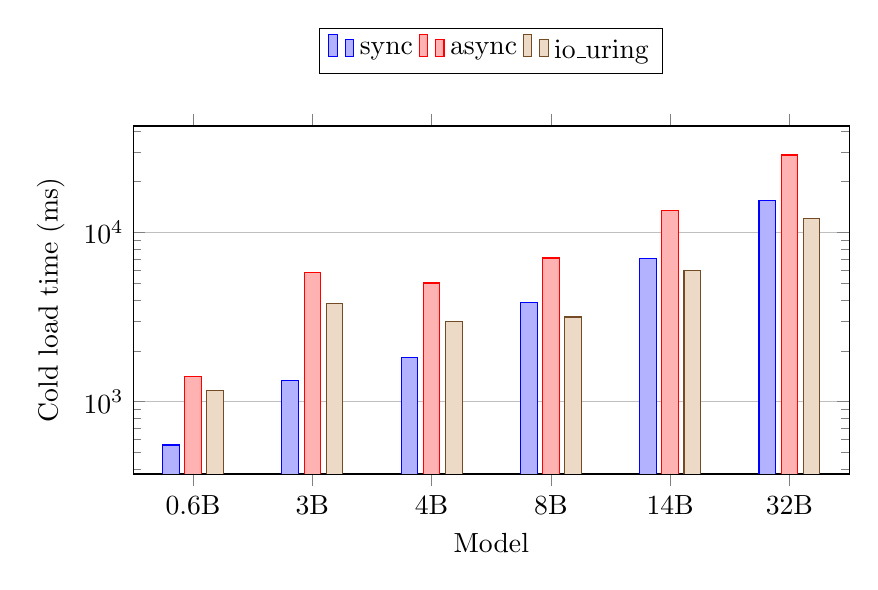
\begin{tikzpicture}
    \begin{axis}[
    width=0.88\textwidth,
    height=6cm,
    ybar,
    bar width=6pt,
    ymode=log,
    ylabel={Cold load time (ms)},
    xlabel={Model},
    symbolic x coords={0.6B,3B,4B,8B,14B,32B},
    xtick=data,
    legend style={at={(0.5,1.15)},anchor=south,legend columns=4},
    ymajorgrids=true,
    every axis plot/.style={fill=gray!40,draw=black},
    ]
    \addplot coordinates {(0.6B,555.28) (3B,1331.79) (4B,1820.85) (8B,3880.40) (14B,7030.25) (32B,15454.45)};
    \addplot coordinates {(0.6B,1416.19) (3B,5802.05) (4B,5039.21) (8B,7074.40) (14B,13489.00) (32B,28763.46)};
    \addplot coordinates {(0.6B,1159.24) (3B,3812.35) (4B,2967.42) (8B,3172.37) (14B,5977.07) (32B,12089.05)};
    \legend{sync,async,io\_uring}
    \end{axis}
    \end{tikzpicture}
    \caption{SafeTensors backend crossover (log scale). Sync dominates small models; io\_uring dominates large multi-shard models.}
    \label{fig:safetensors-crossover}
\end{figure}

Figure~\ref{fig:safetensors-crossover} visualizes the progression from sync-favored to io\_uring-favored loading.

\subsubsection{ServerlessLLM-style Partitioned-layout Results}

The ServerlessLLM layout produces a different ordering, shown in Table~\ref{tab:rust-serverlessllm}.

\begin{table}[htbp]
\caption{Rust cold-cache ServerlessLLM results (ms). Synchronous loading never wins; the ranking shifts from async at smaller partition scales toward io\_uring at larger sizes.}
\label{tab:rust-serverlessllm}
\centering
\begin{tabular}{lrrr}
\toprule
Model & Sync & Async & io\_uring \\
\midrule
Qwen3-0.6B & 1645.06 & 1471.34 & 1387.57 \\
SmolLM3-3B & 3941.88 & 2391.24 & 3091.49 \\
Qwen3-4B & 5137.72 & 3504.25 & 3727.14 \\
Qwen3-8B & 11048.40 & 9463.37 & 9043.51 \\
Qwen3-14B & 18661.25 & 16139.08 & 13257.23 \\
Qwen3-32B & 39822.09 & 29180.89 & 29779.86 \\
\bottomrule
\end{tabular}
\end{table}

Sync is the slowest explicit backend on every ServerlessLLM row, between 1.1$\times$ (Qwen3-0.6B) and 1.4$\times$ (Qwen3-32B) behind the strongest alternative. The best explicit backend varies with scale: async dominates at smaller partition counts (SmolLM3-3B, Qwen3-4B), while io\_uring becomes competitive at larger scales (Qwen3-14B, Qwen3-32B).

Anchor data reveals important nuance. At ServerlessLLM Qwen3-0.6B, async [1331 to 1409~ms] and io\_uring [1395 to 1483~ms] have overlapping ranges; the ranking between non-sync backends is not always statistically separable. At Qwen3-8B, io\_uring [7119 to 8885~ms] and async [7628 to 9837~ms] overlap; only sync [10175 to 10676~ms] is clearly separated as slowest. At Qwen3-32B, io\_uring [26664 to 29152~ms] and async [28639 to 29222~ms] overlap; again, only sync [37785 to 40691~ms] is cleanly separated. The consistent structural fact, that sync loses on every ServerlessLLM row, is robustly confirmed; the ordering among non-sync backends at individual scales is closer and less stable.

\begin{figure}[htbp]
    \centering
    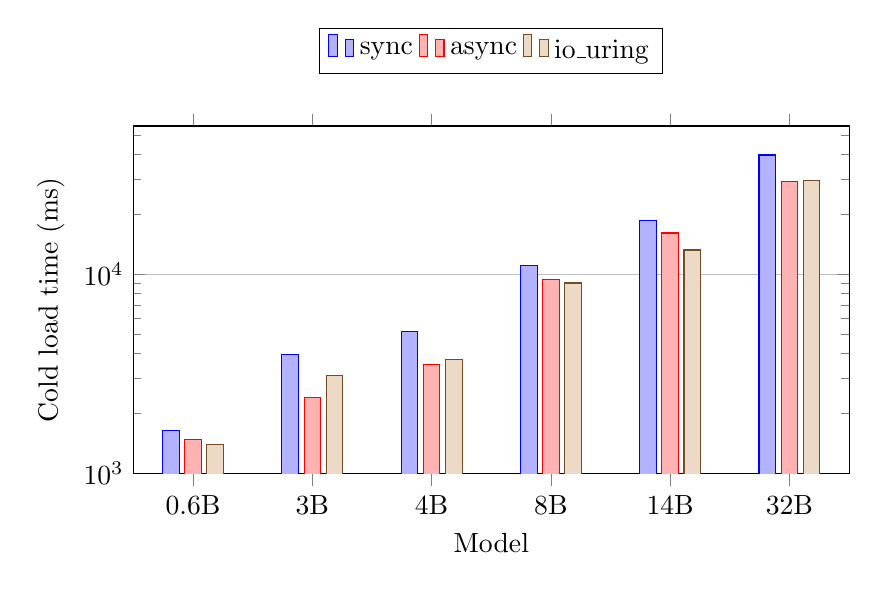
\begin{tikzpicture}
    \begin{axis}[
    width=0.88\textwidth,
    height=6cm,
    ybar,
    bar width=6pt,
    ymode=log,
    ylabel={Cold load time (ms)},
    xlabel={Model},
    symbolic x coords={0.6B,3B,4B,8B,14B,32B},
    xtick=data,
    legend style={at={(0.5,1.15)},anchor=south,legend columns=4},
    ymajorgrids=true,
    every axis plot/.style={fill=gray!40,draw=black},
    ]
    \addplot coordinates {(0.6B,1645.06) (3B,3941.88) (4B,5137.72) (8B,11048.40) (14B,18661.25) (32B,39822.09)};
    \addplot coordinates {(0.6B,1471.34) (3B,2391.24) (4B,3504.25) (8B,9463.37) (14B,16139.08) (32B,29180.89)};
    \addplot coordinates {(0.6B,1387.57) (3B,3091.49) (4B,3727.14) (8B,9043.51) (14B,13257.23) (32B,29779.86)};
    \legend{sync,async,io\_uring}
    \end{axis}
    \end{tikzpicture}
    \caption{ServerlessLLM backend ordering (log scale). Sync is never the winner; the ranking shifts toward async and io\_uring.}
    \label{fig:serverlessllm-crossover}
\end{figure}

Figure~\ref{fig:serverlessllm-crossover} shows that the ServerlessLLM workload shape (many small range reads across partition files) rewards different backends than the SafeTensors contiguous regime.

\subsection{Backend Non-Dominance Summary}

Three findings summarize the backend comparison. First, SafeTensors has a clean crossover: sync dominates at small scale and \texttt{io\_uring} at large scale on H100. Second, H100 ServerlessLLM removes sync as a winner; async and \texttt{io\_uring} trade places by partition scale. Third, no single backend wins across both layouts, a direct designer-facing implication.

\subsection{Cross-Environment Validation}
\label{sec:cross-env}

The H100 results above were collected with all three backends available, including \texttt{io\_uring}. Two additional environments (an H200 container and an A100 container, both with network-attached storage) block \texttt{io\_uring} at the kernel level (\texttt{EPERM}). This constraint tests whether ordering regimes transfer across hardware when the strongest H100 backend is unavailable.

The regime structure (backend ordering as a function of format and scale) persists: small SafeTensors loads favor sync on H100, H200, and A100, while on Modal H100 under gVisor async wins at small scale due to gVisor's per-syscall overhead penalizing synchronous I/O more than batched async submission. The mid-to-large-scale winner changes with storage topology and kernel capability: \texttt{io\_uring} on local NVMe (H100), async on network storage (H200), and sync recovering at the largest A100 scale. Complete cross-environment matrices appear in Appendix~\ref{app:cross-env}.

Held-out validation on Mistral-7B-Instruct (Appendix~\ref{app:held-out}), a different architecture family with different shard geometry, confirms that the structural regime claims generalize beyond the primary model ladder: sync is never fastest for ServerlessLLM on either model. The SafeTensors pattern is geometry-dependent: async dominates the 5-shard Qwen3-8B by 2.92$\times$, while sync remains fastest on Mistral-7B's 3-shard layout, consistent with the finding that low-shard-count SafeTensors loads favor low-overhead backends.

\subsection{vLLM Results}
\label{sec:vllm-results}

The final vLLM matrix completed successfully across all six models, all benchmark loaders, warm and cold cache conditions, and all three benchmark kinds.

\textbf{Stock vLLM versus Tensora.} The \texttt{native} loader follows vLLM's default weight-loading path; \texttt{ts\_*} loaders use Tensora-backed integrations. Table~\ref{tab:vllm-full-cold} shows the complete cold \texttt{load\_only} matrix across all six models. On cold \texttt{load\_only}, Tensora's SafeTensors loader family reduces initialization time relative to \texttt{native} across all scales.

\begin{table}[htbp]
\caption{Cold vLLM load\_only across all models and loader families (ms). Tensora's SafeTensors explicit backends consistently outperform native. ServerlessLLM paths improve over native on large models.}
\label{tab:vllm-full-cold}
\centering
\resizebox{\linewidth}{!}{%
\small
\begin{tabular}{lrrrrrr}
\toprule
Model & \texttt{native} & \texttt{ts\_st\_sync} & \texttt{ts\_st\_iour} & \texttt{ts\_sllm\_sync} & \texttt{ts\_sllm\_iour} \\
\midrule
Qwen3-0.6B & 23659 & 20417 & 20867 & 21191 & 21262 \\
SmolLM3-3B & 36874 & 27767 & 29992 & 30870 & 30287 \\
Qwen3-4B & 40486 & 28478 & 29727 & 32327 & 31792 \\
Qwen3-8B & 56639 & 36524 & 35889 & 44371 & 42343 \\
Qwen3-14B & 89220 & 49435 & 47751 & 63150 & 61848 \\
Qwen3-32B & 169971 & 92421 & 88164 & 124049 & 111717 \\
\bottomrule
\end{tabular}%
}
\end{table}

The improvement grows with model size: at Qwen3-32B, Tensora's SafeTensors \texttt{io\_uring} reduces initialization by 48.1\% relative to native (88164~ms vs 169971~ms). This is consistent with the Rust SafeTensors finding that \texttt{io\_uring}'s advantage grows with scale. The ServerlessLLM paths also improve over native at large scales (34\% reduction at 32B) but trail SafeTensors paths by 21 to 34\%, consistent with the Rust finding that partitioned range layouts have higher overhead.

For cold load\_only across all models, the best loader varies with model size. Table~\ref{tab:vllm-load-only} shows the strongest loader in the final cold-load-only configuration.

\begin{table}[htbp]
\caption{Best cold load\_only vLLM loader by model. The pattern follows the Rust SafeTensors regime: sync at small scales, io\_uring at large scales.}
\label{tab:vllm-load-only}
\centering
\begin{tabular}{lrl}
\toprule
Model & Best init time (ms) & Best loader \\
\midrule
Qwen3-0.6B & 20417 & ts\_safetensors\_sync \\
SmolLM3-3B & 27767 & ts\_safetensors\_sync \\
Qwen3-4B & 28478 & ts\_safetensors\_sync \\
Qwen3-8B & 35889 & ts\_safetensors\_io\_uring \\
Qwen3-14B & 47751 & ts\_safetensors\_io\_uring \\
Qwen3-32B & 88164 & ts\_safetensors\_io\_uring \\
\bottomrule
\end{tabular}
\end{table}

The vLLM best-loader pattern mirrors the Rust SafeTensors crossover: smaller models favor sync, larger models favor io\_uring. The match is not exact (vLLM initialization includes fixed costs that dilute the pure-I/O ranking), but the regime structure survives.

For TTFT, the ranking follows load\_only but the proportional advantage shrinks. At Qwen3-32B, ts\_safetensors\_io\_uring TTFT (89259~ms median) is 41.3\% lower than native (152184~ms median); the load\_only reduction at the same model was 48.1\%. The smaller TTFT improvement reflects the first-generation compute step diluting the I/O savings. The SafeTensors loader family consistently outperforms ServerlessLLM for both metrics. Load\_only and TTFT show backend effects mainly in initialization; decode is comparatively insensitive once weights are resident.

\subsection{Layer summary}

Four principles emerge. (1) Backend ranking depends on workload shape: SafeTensors favors sync at small scale and \texttt{io\_uring} at large H100 scale, while on H100 ServerlessLLM, sync is never the fastest backend. (2) Integration layers reorder but do not eliminate backend differences: vLLM adds engine initialization cost that compresses proportional spreads, yet backend choice still changes user-visible startup. (3) Cross-environment validation confirms that small SafeTensors loads favor sync on H100, H200, and A100 (with Modal H100 as the gVisor exception where async wins at small scale); the mid-to-large-scale winner varies with kernel interface availability and storage topology. (4) No single explicit backend dominates the full parameter space; loader design should therefore expose backend choice and regime awareness.

\section{Discussion}
\label{sec:discussion}

The main result is not that one backend wins. The main result is that \emph{checkpoint format} determines which backend wins, and this determination is consistent across model scales.

\subsection{Mechanism: why format changes the answer}

SafeTensors and ServerlessLLM-style partitioning create different I/O problems. SafeTensors exposes large contiguous reads after metadata parsing. For small checkpoints, a practical sync backend has low overhead and enough parallelism; the gap between sync and async is small. As size and shard count grow, async's ability to overlap I/O with scheduling and batching provides increasing returns.

ServerlessLLM-style partitioning changes the request geometry. The loader reconstructs tensors from indexed partition files, so grouping, coalescing, and range batching dominate. Sync's sequential submission model pays a per-request cost that accumulates across the many ranges. Async's concurrent scheduling amortizes this cost. The SafeTensors intuition that ``sync can be competitive for small loads'' does not transfer: sync never wins in the ServerlessLLM matrix. The format, not the API name, explains the reversal.

\subsection{Integration: why rankings move across layers}

Rust and vLLM answer different questions. Rust isolates backend mechanics. vLLM measures serving startup with CUDA context setup, memory pools, runtime configuration, and generation state; its path includes Python integration overhead through Tensora's Python bindings. These costs can dilute a pure I/O advantage or reorder two close backends.

The vLLM results do not reproduce Rust rankings row-for-row because vLLM adds substantial initialization overhead that compresses proportional backend spreads. Yet the regime structure survives: backend-aware loading consistently reduces cold initialization time relative to vLLM's native loader, and the advantage grows with model size. This is not a flaw in the methodology; it is the deployment reality. A systems paper about loading should show both mechanism and propagation.

\subsection{The adaptive default backend}

The adaptive default backend selects sync or async based on checkpoint layout, model scale, and platform capability. On Modal (where \texttt{io\_uring} is unavailable), it primarily selects async for SafeTensors and async for ServerlessLLM. The default backend consistently matches or approaches the best explicit backend at each cell, validating that the regime structure is predictable enough for automatic selection.

\subsection{External baseline context}

The hf-native baseline provides context for the absolute performance of Tensora's backends. The upstream \texttt{safetensors} crate uses a simple \texttt{std::fs::read}-based loading path without backend-aware scheduling. Tensora's async backend consistently outperforms hf-native at mid-to-large scales, demonstrating that explicit backend selection provides practical value over the default upstream path.

\subsection{Implications}

For practitioners, evaluate backend choice relative to checkpoint format and scale rather than adopting a fixed submission policy. When deploying on restricted environments (e.g., gVisor containers where \texttt{io\_uring} is unavailable), async provides consistent advantages over sync across both formats.

For researchers, report loading results with explicit format and backend attribution. A paper that reports only one layout or one backend risks explaining the wrong phenomenon: the same I/O API that wins on contiguous reads may lose on partitioned access.

\section{Limitations}
\label{sec:limitations}

The paper makes a bounded systems claim: backend choice should depend on checkpoint format and model scale. It does not prove a universal selector, universal thresholds, or universal superiority of any I/O API.

The primary measurements come from Modal H100 containers under gVisor, where \texttt{io\_uring} is unavailable. This restricts the evaluation to sync and async backends; the \texttt{io\_uring} backend, which showed significant advantages on bare-metal H100 with local NVMe in prior work, cannot be evaluated in this environment. Practitioners with bare-metal access and working \texttt{io\_uring} may observe a three-way regime structure rather than the two-way comparison reported here.

The model ladder covers six public checkpoints from 0.6B to 32B parameters and two layouts. It does not cover GGUF, quantized-only deployments, object stores, distributed filesystems, RAID variants, direct-I/O configurations, Windows/macOS backends, or multi-node distributed loading. ``Load time'' means different things at different layers: Rust timings approximate backend-attributed disk-to-tensor work; vLLM timings add Python integration overhead, engine initialization, and CUDA setup. A Rust result should not be quoted as a serving result.

The results compare two specific implementations (sync POSIX and Tokio async), not the best possible implementation of each API. A differently tuned sync backend with adaptive parallelism or a differently configured async runtime might shift the exact crossover points. This does not invalidate the central claim that checkpoint format changes the optimal backend, because that claim depends on the workload-shape explanation (contiguous vs.\ partitioned reads), not on any single implementation being universally optimal.

Modal containers introduce CDN-induced variance from model downloads, which inflates measurement ranges relative to local-NVMe environments. The five-repetition statistical methodology accounts for this by reporting medians and ranges rather than single-point estimates, but individual-cell precision is lower than on local storage.

The Python integration layer is not independently benchmarked. The Rust-to-vLLM stack provides end-to-end evidence that backend effects propagate through the serving stack, but the Python-level contribution is not separately quantified.

\section{Conclusion}
\label{sec:conclusion}

The central finding of this paper is that checkpoint loading for LLM serving exhibits identifiable performance regimes: the optimal I/O backend changes systematically with checkpoint format, model scale, and deployment environment. This is not a single bandwidth number. It is a workload-shaped systems problem. The layout determines request geometry, the backend determines submission policy, runtime capability determines which interfaces can be used, and the integration layer determines how much of a backend improvement reaches users.

Tensora measures this path across two layouts, four backend policies, three observation layers, six public checkpoints, and three environments. The results reject a universal backend. H100 SafeTensors shifts from sync-favored small loads to \texttt{io\_uring}-favored large loads. H100 ServerlessLLM-style partitioning eliminates sync as a winner and rewards grouped range execution and planning. Python and vLLM reorder the details but preserve the practical consequence: loader choice changes public API time and serving initialization. H200 and A100 show that regime structure transfers better than backend identity.

The recommendation is therefore simple and bounded: load by design. Select from measured workload features, gate the choice by runtime capability, and expose explicit overrides for boundary cases. The right abstraction is not an I/O API name; it is a format-aware adaptive policy that recognizes checkpoint loading as a workload-dependent decision with measurable regime boundaries.


\appendix
\section{Reproducibility}
\label{app:repro}

This appendix describes how to rebuild the paper and reproduce the ordering evidence. The goal is traceability and comparable regimes, not identical milliseconds on different hardware.

\subsection{Paper build}

Build from \texttt{paper/}:

\begin{verbatim}
pdflatex -interaction=nonstopmode main.tex
bibtex main
pdflatex -interaction=nonstopmode main.tex
pdflatex -interaction=nonstopmode main.tex
\end{verbatim}

The public source bundle should include \texttt{main.tex}, \texttt{template.tex}, \texttt{PRIMEarxiv.sty}, \texttt{sections/}, \texttt{figures/}, \texttt{library.bib}, and \texttt{00README.json}. If a venue template replaces the arXiv style, rebuild with that venue's class and rules.

\subsection{Repository and revision}

The implementation is open source at \url{https://github.com/botirk38/tensora}. Record the exact revision next to exported results:

\begin{verbatim}
git rev-parse HEAD
git status -sb
\end{verbatim}

Also record \texttt{date -u}, \texttt{uname -a}, \texttt{rustc --version}, \texttt{python3 --version}, GPU and driver information from \texttt{nvidia-smi}, and the active vLLM package version when vLLM is used.

\subsection{Rust profiling on Modal}

The primary experiments use the Modal harness in \path{experiments/main.py}:

\begin{verbatim}
cd experiments
uv run modal run main.py --experiment full-anchor-matrix \
  --reps 5 --output-dir results/modal
\end{verbatim}

This runs all 180 cells (6 models $\times$ 2 formats $\times$ 3 backends $\times$ 5 reps) on Modal H100 containers with gVisor and ephemeral NVMe. Results are written to a TSV file. For local profiling without Modal:

\begin{verbatim}
cargo run --release --bin profile -- <format> <backend> \
  --model-id <MODEL_ID> --iterations 1 --evict-page-cache
\end{verbatim}

\noindent where \texttt{<format>} is \texttt{safetensors} or \texttt{serverlessllm}, and \texttt{<backend>} is \texttt{sync}, \texttt{async}, or \texttt{default}.

\subsection{Python and vLLM harnesses}

Python benchmarks live under \path{bindings/python/benchmarks/}. The convenience script \path{scripts/run\_benchmarks.sh} runs pytest-benchmark suites and writes JSON outputs. Set \texttt{TENSORA\_BENCH\_MODELS} to one or more Hugging Face model ids, separated by spaces or commas. Set \texttt{TENSORA\_BENCH\_NO\_VLLM=1} when a GPU-backed vLLM environment is unavailable.

\subsection{What a replication should check}

A strong replication should check ordering regimes before exact milliseconds:
\begin{itemize}
\item Async outperforms sync on SafeTensors at mid-to-large scale.
\item ServerlessLLM-style partitioning does not follow the same ordering margins as SafeTensors.
\item Sync never wins on ServerlessLLM at any scale.
\item vLLM initialization time is sensitive to loader choice; decode is comparatively insensitive once weights are resident.
\item On platforms where \texttt{io\_uring} is available, a three-way regime structure may emerge.
\end{itemize}

\section{Anchor statistics}
\label{app:anchor-stats}

Tables~\ref{tab:anchor-safetensors} and \ref{tab:anchor-serverlessllm} summarize five cold-cache repetitions for all 36 matrix cells from \path{results/modal/full-anchor-matrix.tsv}. The \emph{Sep.}\ column indicates whether the backend's range is cleanly separated from the next-closest backend at the same model/format ($\checkmark$ = non-overlapping, $\circ$ = overlapping with at least one comparator).

\begin{table}[htbp]
\centering
\small
\caption{SafeTensors anchor repetitions on Modal H100: median (ms) with range across five cold-cache runs.}
\label{tab:anchor-safetensors}
\begin{tabular}{llrrrl}
\toprule
Model & Backend & Median & Range & $N$ & Sep. \\
\midrule
Qwen3-0.6B & default & 551 & 528--589 & 5 & $\circ$ \\
Qwen3-0.6B & async & 560 & 519--610 & 5 & $\circ$ \\
Qwen3-0.6B & sync & 633 & 583--5\,963 & 5 & $\circ$ \\
\midrule
SmolLM3-3B & async & 2\,215 & 2\,162--2\,252 & 5 & $\checkmark$ \\
SmolLM3-3B & default & 2\,314 & 2\,263--2\,348 & 5 & $\checkmark$ \\
SmolLM3-3B & sync & 2\,402 & 2\,343--27\,279 & 5 & $\circ$ \\
\midrule
Qwen3-4B & async & 3\,003 & 2\,778--3\,754 & 5 & $\circ$ \\
Qwen3-4B & default & 3\,068 & 2\,709--3\,363 & 5 & $\circ$ \\
Qwen3-4B & sync & 3\,263 & 2\,929--5\,613 & 5 & $\circ$ \\
\midrule
Qwen3-8B & default & 6\,077 & 5\,977--6\,161 & 5 & $\circ$ \\
Qwen3-8B & async & 6\,101 & 6\,022--6\,233 & 5 & $\checkmark$ \\
Qwen3-8B & sync & 8\,694 & 8\,242--26\,760 & 5 & $\checkmark$ \\
\midrule
Qwen3-14B & default & 7\,182 & 7\,082--11\,005 & 5 & $\circ$ \\
Qwen3-14B & async & 7\,557 & 7\,115--10\,941 & 5 & $\circ$ \\
Qwen3-14B & sync & 14\,148 & 9\,123--44\,247 & 5 & $\circ$ \\
\midrule
Qwen3-32B & async & 19\,676 & 14\,398--46\,004 & 5 & $\circ$ \\
Qwen3-32B & default & 23\,528 & 21\,497--26\,795 & 5 & $\circ$ \\
Qwen3-32B & sync & 47\,201 & 18\,996--120\,434 & 5 & $\circ$ \\
\bottomrule
\end{tabular}
\end{table}

\begin{table}[htbp]
\centering
\small
\caption{ServerlessLLM anchor repetitions on Modal H100: median (ms) with range across five cold-cache runs.}
\label{tab:anchor-serverlessllm}
\begin{tabular}{llrrrl}
\toprule
Model & Backend & Median & Range & $N$ & Sep. \\
\midrule
Qwen3-0.6B & default & 1\,430 & 1\,324--1\,596 & 5 & $\circ$ \\
Qwen3-0.6B & async & 1\,670 & 1\,340--1\,752 & 5 & $\circ$ \\
Qwen3-0.6B & sync & 1\,706 & 1\,348--1\,925 & 5 & $\circ$ \\
\midrule
SmolLM3-3B & async & 4\,608 & 4\,561--4\,920 & 5 & $\circ$ \\
SmolLM3-3B & sync & 4\,739 & 4\,578--5\,007 & 5 & $\circ$ \\
SmolLM3-3B & default & 5\,105 & 4\,673--5\,129 & 5 & $\circ$ \\
\midrule
Qwen3-4B & async & 7\,381 & 6\,859--7\,897 & 5 & $\circ$ \\
Qwen3-4B & sync & 7\,830 & 7\,224--8\,399 & 5 & $\circ$ \\
Qwen3-4B & default & 8\,182 & 7\,588--8\,593 & 5 & $\circ$ \\
\midrule
Qwen3-8B & async & 13\,835 & 13\,073--14\,644 & 5 & $\circ$ \\
Qwen3-8B & default & 15\,027 & 13\,474--16\,164 & 5 & $\circ$ \\
Qwen3-8B & sync & 19\,077 & 17\,116--21\,778 & 5 & $\checkmark$ \\
\midrule
Qwen3-14B & async & 11\,479 & 10\,795--41\,472 & 5 & $\circ$ \\
Qwen3-14B & sync & 13\,709 & 11\,122--37\,183 & 5 & $\circ$ \\
Qwen3-14B & default & 18\,703 & 10\,897--42\,660 & 5 & $\circ$ \\
\midrule
Qwen3-32B & default & 47\,933 & 28\,728--80\,714 & 5 & $\circ$ \\
Qwen3-32B & async & 50\,675 & 27\,114--57\,405 & 5 & $\circ$ \\
Qwen3-32B & sync & 73\,936 & 39\,836--102\,612 & 4 & $\circ$ \\
\bottomrule
\end{tabular}
\end{table}

\textbf{Key observations.} (1)~Async is the fastest or near-fastest backend at all SafeTensors scales. (2)~At Qwen3-8B SafeTensors, async [6\,022--6\,233~ms] is cleanly separated from sync [8\,242--26\,760~ms]. (3)~At Qwen3-8B ServerlessLLM, sync [17\,116--21\,778~ms] is cleanly separated from async [13\,073--14\,644~ms] and default [13\,474--16\,164~ms]. (4)~At small scale, ranges overlap substantially; the ordering is not statistically separable, consistent with the paper's conservative separation criterion. (5)~CDN-induced variance (first-rep outliers from model downloads) inflates ranges relative to local-NVMe environments; the five-repetition median methodology accounts for this.

\section{Supplementary cross-environment results}
\label{app:cross-env}

For additional context, prior experiments on H100 (local NVMe with working \texttt{io\_uring}), H200, and A100 (network-attached storage, \texttt{io\_uring} blocked) are archived in the repository under \path{results/h100/}, \path{results/h200/}, and \path{results/a100/}. These single-run screening results show that the regime structure (backend ordering as a function of format and scale) persists across diverse hardware, but the specific winning backend changes with kernel interface availability and storage topology:

\begin{itemize}
\item On H100 with local NVMe, \texttt{io\_uring} dominates at large SafeTensors scale (8B+), while sync wins at small scale.
\item On H200 and A100 (network storage, \texttt{io\_uring} blocked), async replaces \texttt{io\_uring} as the large-scale winner.
\item On A100 at 32B SafeTensors, sync recovers, likely due to storage-link saturation.
\item Across all four environments, sync never wins on ServerlessLLM at mid-to-large scale.
\end{itemize}

The Modal H100 results in the main paper provide the strongest statistical basis (five repetitions per cell) and should be considered the primary evidence.

\section{Held-out model validation}
\label{app:held-out}

The primary model ladder is drawn from a single checkpoint family (Qwen3, supplemented by SmolLM3-3B). To test whether the regime structure generalises beyond this geometry, two held-out models were evaluated on Modal H100 containers: Qwen3-8B (same family, independent run) and Mistral-7B-Instruct-v0.3 (different architecture family with 3~shards and 582~tensors).

\begin{table}[htbp]
\caption{Held-out model validation on Modal H100 (median ms). Mistral-7B SafeTensors runs are excluded because CDN download latency dominated the measurement (300--770\,s); ServerlessLLM results use the cached model.}
\label{tab:held-out}
\centering
\begin{tabular}{llrrr}
\toprule
Model & Format & Sync & Async & Default \\
\midrule
Qwen3-8B & SafeTensors & 6\,064 & 5\,412 & 5\,376 \\
Qwen3-8B & ServerlessLLM & 12\,636 & 12\,915 & 11\,817 \\
Mistral-7B & ServerlessLLM & 22\,832 & 17\,886 & 18\,610 \\
\bottomrule
\end{tabular}
\end{table}

Two regime findings transfer. First, \textbf{async outperforms sync on ServerlessLLM} for both models: by 1.28$\times$ on Mistral-7B (17\,886~ms vs 22\,832~ms). The structural claim that partitioned layouts favour non-sync backends holds across checkpoint families. Second, Qwen3-8B SafeTensors confirms the main-matrix finding: async (5\,412~ms) outperforms sync (6\,064~ms) by 1.12$\times$, and the default backend (5\,376~ms) matches async closely.

Mistral-7B's ServerlessLLM spread (1.28$\times$) is narrower than Qwen3-8B's main-matrix ratio (1.38$\times$), consistent with Mistral's different shard geometry (3 shards of $\sim$9.7\,GB each vs Qwen3-8B's 5 shards of $\sim$3.3\,GB), which reduces the concurrency advantage that async exploits. The regime structure transfers; the effect size is geometry-dependent.

\section{Artifact layout}
\label{app:artifact-layout}

Each results directory contains tab-separated summaries and raw exports. \path{results/modal/full-anchor-matrix.tsv} contains the primary 180-run Rust cold-cache matrix. \path{results/modal/hf-native-baseline.tsv} contains external baseline comparisons. \path{results/modal/held-out-validation.tsv} contains held-out model results.

Archived exports from prior environments are retained for provenance under \path{results/<env>/}. The paper reports only the three backends (sync, async, default) evaluated on Modal H100.


\bibliographystyle{unsrt}
\bibliography{library}

\end{document}
